\gdef\thisproblemauthor{}
\gdef\thisproblemdeveloper{}
\gdef\thisproblemorigin{}
\begin{problem}{餐桌禮儀}
{standard input}{standard output}
{1 seconds}{512 MB}{}

跑出洞穴外的Sana迷路了,孤獨的她在人來人往的街道上逗留,十分的可憐,不過此時有一個好心的老爺爺看她在街上餓著肚子,因此招待她一起吃個晚餐,順便等警察到來。

\centerline{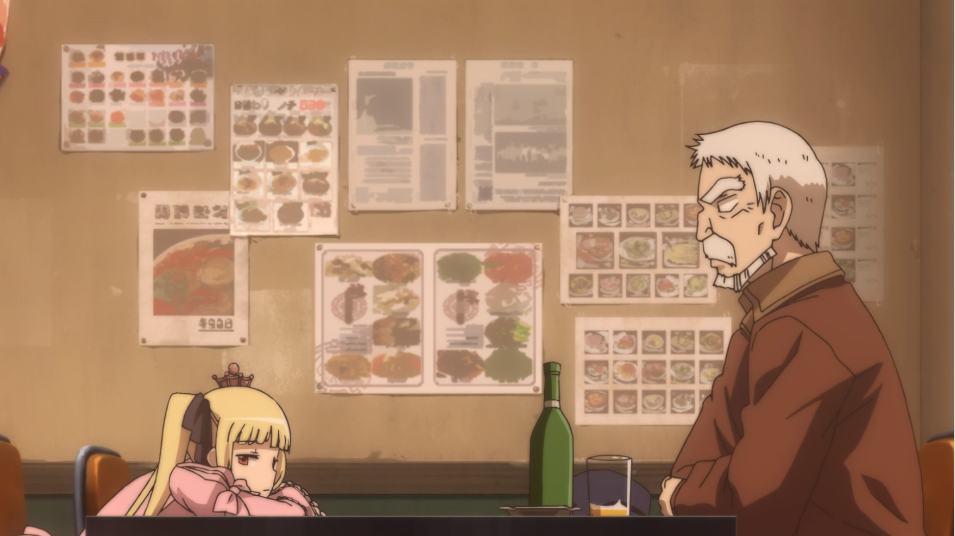
\includegraphics[scale=0.4]{./pics/C.png}}

在老爺爺家,除了Sana還有$N$個人要吃晚餐,身為傳統的東方家庭,使用筷子吃飯是理所當然的,不過老爺爺家的筷子因多年的使用,每支筷子的長度都不太一樣,而且每一個人吃飯時,老爺爺都會發給每個人\textbf{三隻}筷子,多出來最長的那一隻可以當叉子使用,較短的兩隻則做為一般的筷子使用。不過因為筷子的長度參差不齊,拿在手上會有不適感,若兩隻長度為$a,b$的筷子拿在手上,會造成$(a-b)^2$的不適分數。好奇的Sana知道了所有筷子的長度,能幫她計算老爺爺發完筷子之後,所有人不適分數總和最小是多少嗎?

\InputFile

有多筆測資,但是不超過$50$筆測資。測資第一行有兩個整數$N,K$,表示老爺爺家有$N$個人,總共有$K$隻筷子。接下來下一行有$K$個數字,第i個數字$a_i$表示第$i$隻筷子的長度。

\begin{iofmt}
\begin{itemize}
	\item $1\leq N \leq 1000$
	\item $3N+3\leq K \leq 5000$
	\item $1 \leq a_i \leq 30000$
	\item $a_i \leq a_{i+1}$
	\item 有$10$分的測資$N\leq 1$
	\item 有$10$分的測資$K\leq 20$
	\item 有$30$分的測資$N\leq 100$
\end{itemize}
\end{iofmt}

\OutputFile

對於每一筆測資輸出一行,為發給每個人筷子後,不適分數可能的最小值。

\Examples

\begin{example}
\exmpfile{./sample/PC.sample.in}{./sample/PC.sample.out}%
\end{example}


\end{problem}
